% !TEX encoding = UTF-8 Unicode
\documentclass[a4paper]{article}

\usepackage{color}
\usepackage{url}
\usepackage[T2A]{fontenc} % enable Cyrillic fonts
\usepackage[utf8]{inputenc} % make weird characters work
\usepackage{graphicx}

\usepackage[english,serbian]{babel}
%\usepackage[english,serbianc]{babel} %ukljuciti babel sa ovim opcijama, umesto gornjim, ukoliko se koristi cirilica

\usepackage[unicode]{hyperref}
\hypersetup{colorlinks,citecolor=green,filecolor=green,linkcolor=blue,urlcolor=blue}

\usepackage{listings}

%\newtheorem{primer}{Пример}[section] %ćirilični primer
\newtheorem{primer}{Primer}[section]

\definecolor{mygreen}{rgb}{0,0.6,0}
\definecolor{mygray}{rgb}{0.5,0.5,0.5}
\definecolor{mymauve}{rgb}{0.58,0,0.82}

\lstset{ 
  backgroundcolor=\color{white},   % choose the background color; you must add \usepackage{color} or \usepackage{xcolor}; should come as last argument
  basicstyle=\scriptsize\ttfamily,        % the size of the fonts that are used for the code
  breakatwhitespace=false,         % sets if automatic breaks should only happen at whitespace
  breaklines=true,                 % sets automatic line breaking
  captionpos=b,                    % sets the caption-position to bottom
  commentstyle=\color{mygreen},    % comment style
  deletekeywords={...},            % if you want to delete keywords from the given language
  escapeinside={\%*}{*)},          % if you want to add LaTeX within your code
  extendedchars=true,              % lets you use non-ASCII characters; for 8-bits encodings only, does not work with UTF-8
  firstnumber=1000,                % start line enumeration with line 1000
  frame=single,	                   % adds a frame around the code
  keepspaces=true,                 % keeps spaces in text, useful for keeping indentation of code (possibly needs columns=flexible)
  keywordstyle=\color{blue},       % keyword style
  language=Python,                 % the language of the code
  morekeywords={*,...},            % if you want to add more keywords to the set
  numbers=left,                    % where to put the line-numbers; possible values are (none, left, right)
  numbersep=5pt,                   % how far the line-numbers are from the code
  numberstyle=\tiny\color{mygray}, % the style that is used for the line-numbers
  rulecolor=\color{black},         % if not set, the frame-color may be changed on line-breaks within not-black text (e.g. comments (green here))
  showspaces=false,                % show spaces everywhere adding particular underscores; it overrides 'showstringspaces'
  showstringspaces=false,          % underline spaces within strings only
  showtabs=false,                  % show tabs within strings adding particular underscores
  stepnumber=2,                    % the step between two line-numbers. If it's 1, each line will be numbered
  stringstyle=\color{mymauve},     % string literal style
  tabsize=2,	                   % sets default tabsize to 2 spaces
  title=\lstname                   % show the filename of files included with \lstinputlisting; also try caption instead of title
}

\begin{document}

\title{Pouzdanost softvera\\ \small{Seminarski rad u okviru kursa\\Metodologija stručnog i naučnog rada\\ Matematički fakultet}}

\author{Nenad Ajvaz, Stefan Kapunac, Filip Jovanović, Aleksandra Radosavljević\\ nenadajvaz@hotmail.com, stefankapunac@gmail.com, \\jovanovic16942@gmail.com, aleksandraradosavljevic.@live.com}

%\date{9.~april 2015.}

\maketitle

\abstract{
ABSTRAKT ABSTRAKT ABSTRAKT ABSTRAKT ABSTRAKT ABSTRAKT ABSTRAKT ABSTRAKT
ABSTRAKT ABSTRAKT ABSTRAKT ABSTRAKT ABSTRAKT ABSTRAKT ABSTRAKT ABSTRAKT
ABSTRAKT ABSTRAKT ABSTRAKT ABSTRAKT ABSTRAKT ABSTRAKT ABSTRAKT ABSTRAKT
ABSTRAKT ABSTRAKT ABSTRAKT ABSTRAKT ABSTRAKT ABSTRAKT ABSTRAKT ABSTRAKT
ABSTRAKT ABSTRAKT ABSTRAKT ABSTRAKT ABSTRAKT ABSTRAKT ABSTRAKT ABSTRAKT
ABSTRAKT ABSTRAKT ABSTRAKT ABSTRAKT ABSTRAKT ABSTRAKT ABSTRAKT ABSTRAKT
ABSTRAKT ABSTRAKT ABSTRAKT ABSTRAKT ABSTRAKT ABSTRAKT ABSTRAKT ABSTRAKT
}

\tableofcontents

\newpage

\section{Uvod}
\label{sec:uvod}

- Velika uloga softvera u danasnje vreme \\
- Softver je sve rasprostranjeniji, uskoro ce postati osnovna radna snaga \\
- Sa povecanjem uloge softvera u drustvu, njegova pouzdanost ima veci znacaj, jer
od softvera vec uveliko zavise i ljudski zivoti \\
- Za razliku od ljudi, softver ne pravi slucajne greske, ali do gresaka \\
ipak dolazi iz raznih razloga (mali promaci i male greske se vremenom ispoljavaju) \\
- U nastavku cemo predstaviti mere i modele pouzdanosti softvera, metode za poboljsanje pouzdanosti, kao i primere i u kojima su greske u sistemu dovele do ozbiljnih problema


\section{Primeri padova softvera}
\label{sec:primeri}
- Izmedju ostalih, dodati primer za Boing (sad ovaj sto je pao, 10. marta) \\



\section{``Program testing can be used to show the presence of bugs, but never to show their absence!'' - Edsger W. Dijkstra}
\label{sec:dijkstra}
Greške u razvoju softvera su, kao i svuda, neizbežne.
Ne možemo da se nadamo visokom nivou pouzdanosti softvera ako te greške ne pokušamo na neki način da uklonimo.
Dakle, kao što se vidi na slici \ref{fig:rs}, u razvojnom ciklusu softvera testiranje ima izuzetno važnu ulogu.

\begin{figure}[h!]
\begin{center}
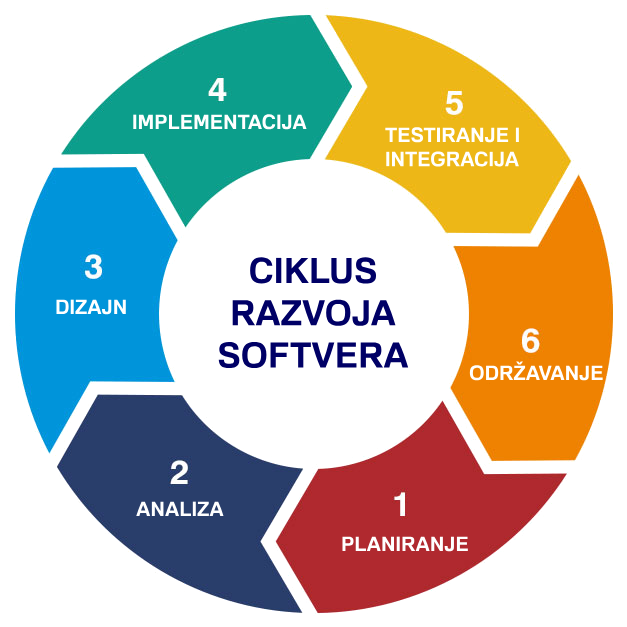
\includegraphics[scale=0.25]{rs.png}
\end{center}
\caption{Ciklus razvoja softvera}
\label{fig:rs}
\end{figure}

\subsection{Ali...}
\label{subsec:ali}
Za skoro svaki, čak i najjednostavniji program postoji ogroman broj mogućih ulaznih vrednosti, tako da je iscrpno testiranje svih mogućnosti praktično neizvodljivo.
Na primer, da bismo testiranjem dokazali ispravnost programa koji sabira dva 64-bitna broja, bilo bi nam potrebno $2^{64} \cdot 2^{64}$ različitih testova.
Uz pretpostavku da jedan test traje jednu nanosekundu, iscrpno testiranje bi trajalo $10^{22}$ godina.
Testiranje je važno i podiže stepen pouzdanosti softvera, pomaže nam da uvidimo da postoje greške u programu, ali gotovo nikada ne možemo samo testiranjem da dokažemo da one ne postoje.

Očigledno nam je potreban bolji pristup za dokazivanje ispravnosti programa.
Grana računarstva koja se time bavi je verifikacija softvera.
Tačnije, proces verifikacije podrazumeva proveru da li program zadovoljava zadatu specifikaciju.
Specifikacija predstavlja model problema i obično sadrži sledeće informacije \cite{laski2009software}:
\begin{itemize}
\item ulazni parametri
\item izlazni parametri
\item globalne promenljive kojima se može pristupiti
\item preduslovi - ograničenja na ulazne vrednosti
\item postuslovi - uslovi koje izlazne vrednosti moraju da zadovolje (za ulaze koji zadovoljavaju preduslove)
\end{itemize}
Verifikacija se sprovodi pod pretpostavkom da je specifikacija validna.
Sa druge strane, validacija proverava da li specifikacija zadovoljava korisničke potrebe.
Razliku između verifikacije i validacije na interesantan način objasnio je Beri Bem:
\begin{quote}
verification = Are we building the product right? \\
validation = Are we building the right product?
\end{quote}

U nastavku ćemo detaljnije objasniti različite vrste verifikacije sofvera, kao i njihov značaj za pouzdanost softvera.

\subsection{Verifikacija softvera}
\label{subsec:verifikacija}
Verifikacija softvera se u osnovi deli na dinamičku i statičku.\\
Dinamička verifikacija podrazumeva ispitivanje korektnosti programa u toku njegovog izvršavanja.
Najčešći oblik dinamičke verifikacije softvera jeste testiranje.\\
Najšira podela testiranja \cite{laski2009software}:
\begin{itemize}
\item testiranje crne kutije\\
Naziva se i funkcionalno testiranje.\\
Testovi se biraju na osnovu specifikacije.
\item testiranje bele kutije\\
Naziva se i strukturno testiranje.\\
Testovi se biraju na osnovu interne strukture koda.
\end{itemize}

Sa druge strane, statička verifikacija podrazumeva analizu izvornog koda programa, na osnovu koje se dolazi do zaključaka o njegovoj korektnosti.
Neke od metoda koje se koriste u statičkoj verifikaciji softvera su:
\begin{itemize}
\item simboličko izvršavanje \cite{symbolic_execution}\\
Koriste se simboličke promenljive umesto stvarnih ulaznih vrednosti, a kao izlaz se dobija simbolički izraz.
\item apstraktna interpretacija \cite{abstract_interpretation}\\
Posmatra se apstraktna semantika, nadskup konkretne semantike programa, u kojoj je rezonovanje jednostavnije.

\end{itemize}

\subsection{Zašto samo odmah ne uradimo sve tačno?}
\label{subsec:formalni_dokazi}
Formalne metode verifikacije softvera podrazumevaju razvoj softvera direktno iz specifikacije i daju matematički dokaz korektnosti programa.
Uz programski kod uporedo se formira i formalan matematički dokaz kojim se obezbeđuje ispravnost, bez potrebe za naknadnim testiranjem.
U te svrhe se koriste alati za interaktivno dokazivanje teorema, kao što su Isabelle/HOL \cite{isabelle} i Coq \cite{coq}.
Ovakvo rešenje je najbolje što se tiče pouzdanosti softvera, jer je matematički dokazana ispravnost.
Međutim, zbog potrebe za stručnjacima koji će to sprovoditi, povećavaju se troškovi, kao i trajanje razvojnog procesa, tako da ne čudi što se u industriji ove metode koriste samo u retkim slučajevima, i to samo za najkritičnije delove koda.\\
Neki od primera formalno verifikovanog softvera su:
\begin{itemize}
\item CompCert - kompilator za programski jezik C \cite{compcert}
\item seL4 - jezgro operativnog sistema (koristi se u avio-industriji) \cite{sel4}
\item CakeML - implementacija programskog jezika ML sa formalno verifikovanim kompilatorom \cite{cakeml}
\item IronFleet - distribuirani sistemi \cite{ironfleet}
\end{itemize}

primer nekog dokaza u izabelu u dodatku...\\



\section{Modeli i metrike pouzdanosti softvera}	
\label{sec:modeli_metrike}

Kao što je prethodno napomenuto, prilikom izgradnje softvera, veoma je važno imati na umu da se greška može naći u bilo kojoj fazi njegovog razvoja. Zato je bitno da se pronađe način procene broja potencijalnih grešaka u sistemu.\\
Statistika pokazuje da se krajem 20. veka na 1000 linija koda pojavi oko 8 grešaka, ne računajući prethodno testiranje sistema. Različiti izvori napominju da je danas taj broj veći, nabraja se 15-50 grešaka na 1000 linija. Majkrosoft tvrdi da njihov kod sadrži 0.5 neispravnosti na istom broj linija, dok NASA čak ni na 500,000 linija programskog koda ne sadrži niti jedan softverski problem \cite{Statistika_prosek_gresaka}. Ovi brojevi su rezulat mnogih spoljašnjih faktora i nisu odgovarajuće merilo propusta i grešaka. Zbog toga su napravljeni razni modeli i metrike koji preciznije daju informaciju o stabilnosti softvera. U nastavku će biti opisana dva tipa takvih modela.\\


\subsection{Deterministički modeli}
\label{sec:deterministicki}

Ovaj model odlikuje preciznim merama i podacima koji se oslanjanju na same karakteristike programskog koda. Prilikom ocenjivanja, ne uzimaju se u obzir slučajni događaji i greške koji oni prouzrokuju, već su performanse računate prema egzaktnim podacima. Oni uključuju broj različitih operatora, operanada, kao i broj mašinskih instrukcija i grešaka. Fokus je na mehanizmu i načinu rada samog softvera, gde se uvek mogu predvideti očekivana stanja.\\
Dva najpoznatija deterministička modela su Holstedova metrika i Mek-Kejbova ciklomatična složenost.\footnote{Moris Hauard Holsted (1977), Tomas Mek-Kejb (1976)}

\subsubsection{Holstedova metrika}
\label{subsec:holsted}

Ova metrika se smatra jednom od najboljih za procenu kompleksnosti softvera, ali i težinu prilikom njegovog testiranja i debagovanja. U obzir ocene implementacije ulazi broj instrukcija i operacija izvornog koda, koji će biti drugačiji za svaki programski jezik ili arhitekturu na kojoj se program izvršava. Uvodi se sledeća notacija:\\

\begin{table}[h]
\centering
 \begin{tabular}{|c|c|c|}
  \hline
  Obeležje & Opis & Formula \\ [0ex] 
  \hline
  $n_1$ & broj jedinstvenih operatora & \\ 
  \hline
  $n_2$ & broj jedinstvenih operanada & \\ 
  \hline
  $n$ & vokabular programa & $ n_1 + n_2 $ \\ 
  \hline
  $N_1$ & ukupan broj operatora & $ n_1 \cdot log_2(n_1) $ \\ 
  \hline
  $N_2$ & ukupan broj operanada & $ n_2 \cdot log_2(n_2) $ \\ 
  \hline
  $N$ & dužina programa & $ N_1 + N_2 $ \\
  \hline
  $I$ & broj mašinskih instrukcija & \\
  \hline
  $V$ & obim programa & $ N \cdot log_2(n_1+n_2) $ \\
  \hline
  $D$ & težina razumevanja i debagovanja & $ n_1/2 \cdot N_2 / 2  $ \\
  \hline
  $M$ & vreme utrošeno na implementaciju & $ V \cdot D $ \\
  \hline
  $T$ & vreme utrošeno na testiranje & $ M / 18 $ \\
  \hline
  $E$ & broj grešaka i bagova & $ V / 3000 $ \\
  \hline
 \end{tabular}
 \caption{Obeležja u Holstedovoj metrici. Brojevi su dobijeni empirijski. \cite{ibm_halstead}}
 \label{tabela:1} 
\end{table}

- TODO:  ubaciti primer iz knjige? 

\subsubsection{Mek-Kejbova ciklomatična složenost}
\label{subsec:mekkejb}

Ova metrika računa složenost dijagrama koji se pravi na osnovu grafa kontrole toka podataka programa. Čvorovi grafa predstavljaju različite komande, a oni su povezani usmerenom granom ako je sledeća naredba prvog čvora ona naredba u drugom čvoru. \\
U slučaju da je graf povezan, ciklomatični broj jednak je broju linearno nezavisnih putanja kroz graf. Jednostavnije rečeno, ako program ne sadrži uslove i grananja, taj broj je 1. Zatim bi se taj broj povećao za 1 svaki put kada se naiđe na neku od ključnih reči: if, while, for, repeat, and, or itd. U naredbi case bi se svaki slučaj posebno računao. Mek-Kejb je za Fortran okruženje odredio da je gornja granica za ciklomatični broj 10, i program se u tom slučaju može smatrati visokog kvaliteta.\\
Ovom metrikom se mogu meriti i manje celine izvornog koda, kao što su pojedinačne funkcije, klase, moduli i potprogrami.\\
Ciklomatični broj C(G) grafa G se računa po formuli:
\begin{center}
C(G) = E - V + 2P,
\end{center}
gde je:\\
E = broj grana grafa\\
V = broj čvorova grafa\\
P = broj povezanih komponenti grafa\\

Ciklomatični broj grafa sa više od jedne povezane komponente se računa kao suma ciklomatičnih brojeva svakih od povezanih komponenti. Kada se merenje vrši nad funkcijom,  P će biti 1, jer funkcija predstavlja jedinstvenu povezanu komponentu.\\
- TODO:  ubaciti primer iz knjige? 

\subsection{Probabilistički modeli}
\label{sec:probabilisticki}

Ovaj model pojavu grešaka i kvarova gleda kao na verovatnosne događaje. Softver se posmatra u fazi izvršavanja i pravi se mreža modela koja predstavlja ponašanje programa. Rezultat ovog modeliranja je primenjiv na razne metode iz oblasti statistike, što omogućava dubinsku matematičku analizu, detekciju anomalija, generisanju testova i simulaciju raznih slučajeva. Postoji nekoliko probabilističkih modela, od kojih će u nastavku biti opisana tri proizvoljna. \\

\subsubsection{Modeli stope neuspeha}
\label{subsec:stopa_neuspeha}

Ova grupa modela se koristi radi prikazivanja kolika je stopa otkazivanja programa po grešci. Kako se broj preostalih grešaka menja, tako se i stopa neuspeha prilagođava promeni.\\
Postoji nekoliko varijacija ovih modela, ali se svi oslanjaju na princip da u kodu postoji \textit{N} međusobno nezavisnih grešaka sa jednakom verovatnoćom ispoljavanja. Kada ona nastane, greška se otklanja i nijedna nova greška se ne pojavljuje prilikom uklanjanja.\\
Razlika je u tome što neki podmodeli podrazumevaju povećanje broja grešaka kroz vreme, drugi podrazumevaju smanjenje, a neki ga smatraju konstantnim. Takođe postoje modeli koji sa sigurnošću tvrde da je greška uklonjena, a postoje i oni koji uspešnost otklanjanja procenjuju verovatnoćom \textit{p}.

\subsubsection{Modeli rasta pouzdanosti}
\label{subsec:rast_pouzdanosti}

- TODO: reliability growth models

\subsubsection{Markovljev model strukture}
\label{subsec:markov}
- TODO: Markov structure models


\section{Budućnost softvera}
\label{buducnost}

- TODO \\

\section{Zaključak}
\label{sec:zakljucak}

- TODO \\

\addcontentsline{toc}{section}{Literatura}
\appendix
\bibliography{seminarski} 
\bibliographystyle{ieeetr}

\appendix
\section{Dodatak}
Ovde pišem dodatne stvari, ukoliko za time ima potrebe.
Ovde pišem dodatne stvari, ukoliko za time ima potrebe.
Ovde pišem dodatne stvari, ukoliko za time ima potrebe.
Ovde pišem dodatne stvari, ukoliko za time ima potrebe.
Ovde pišem dodatne stvari, ukoliko za time ima potrebe.


\end{document}
